\documentclass[aps,pra,showpacs,amsmath,amssymb,nofootinbib,longbibliography,superscriptaddress
]{revtex4-1}

%\documentclass[a4paper]{quantumarticle}
%\newcommand{\onlinecite}{\cite}
%\pdfoutput=1
%\usepackage{mcite}
%\usepackage[sort&compress,numbers]{natbib}
%\bibliographystyle{apsrev4-1}


\usepackage[pdftex]{graphicx}
\usepackage[usenames,dvipsnames]{xcolor}
\usepackage{epstopdf}
\usepackage{tikz}    % Include the tikz package for drawing
\usepackage{mathtools}

\usepackage[normalem]{ulem}


\usepackage[utf8]{inputenc}
\usepackage[T1]{fontenc}

\usepackage{beramono}
\usepackage{listings}

\usepackage{lmodern}

\usepackage{amssymb,amsmath,amsthm}

\usepackage{bbm}

\usepackage{subcaption}

\usepackage{algorithm}
\usepackage{algpseudocode}

\usepackage{graphicx}
\usepackage{subcaption}


\usepackage{mathtools}
\DeclarePairedDelimiter\bra{\langle}{\rvert}
\DeclarePairedDelimiter\ket{\lvert}{\rangle}
\DeclarePairedDelimiterX\braket[2]{\langle}{\rangle}{#1\,\delimsize\vert\,\mathopen{}#2}


\usepackage[justification=raggedright,singlelinecheck=false]{caption}

\DeclareMathAlphabet{\mathbbmsl}{U}{bbm}{m}{sl}

\newtheorem{theorem}{Theorem}
\theoremstyle{definition}
\newtheorem{definition}{Definition}

\theoremstyle{remark}
\newtheorem*{remark}{Remark}

\newtheorem{corollary}{Corollary}[theorem]
\newtheorem{lemma}[theorem]{Lemma}
\renewcommand{\qedsymbol}{$\blacksquare$}

\renewcommand{\lstlistingname}{Code Block}

\newcommand{\patbox}[1]{\vspace{2mm}\noindent\fbox{\parbox{0.47\textwidth}{\hspace{1mm}\parbox{\columnwidth}{\hspace{1mm}\\#1\vspace{1.5mm}}}}\\}

\lstdefinelanguage{julia}%
  {morekeywords={abstract,break,case,catch,const,continue,do,else,elseif,%
      end,export,false,for,function,immutable,import,importall,if,in,%
      macro,module,otherwise,quote,return,switch,true,try,type,typealias,%
      using,while},%
   sensitive=true,%
   alsoother={\$},%
   morecomment=[l]\#,%
   morecomment=[n]{\#=}{=\#},%
   morestring=[s]{"}{"},%
   morestring=[m]{'}{'},%
     literate={é}{{\'e}}1
           {è}{{\`e}}1
           {ù}{{\`u}}1
}[keywords,comments,strings]%

\lstset{%
    language          = julia,
    basicstyle        = \ttfamily,
    keywordstyle      = \bfseries\color{blue},
    numbers           = left,
    numbers           = none,
    stringstyle       = \color{magenta},
    commentstyle      = \color{ForestGreen},
    showstringspaces  = false,
    frame             = single, 
    inputencoding     = latin1,
    breaklines        = true,
    breakatwhitespace = true
}

\newcommand{\FRrefsec}[1]{sec.~\ref{#1}}
\newcommand{\FRreffig}[1]{fig.~\ref{#1}}
\newcommand{\FRrefeq}[1]{eq.~\ref{#1}}

\newcommand{\ENrefsec}[1]{Sec.~\ref{#1}}
\newcommand{\ENreffig}[1]{Fig.~\ref{#1}}
\newcommand{\ENrefeq}[1]{Eq.~\ref{#1}}



\newcommand{\Ham}{\hat{\mathcal{H}}}
\newcommand{\Spin}{\hat{S}}
\newcommand{\A}{\hat{A}{}}
\newcommand{\B}{\hat{B}{}}
\newcommand{\M}{\hat{M}}
\newcommand{\densmat}{\hat{\rho}}
\newcommand{\U}{\hat{U}{}}
\newcommand{\D}{\hat{D}{}}
\newcommand{\V}{\hat{V}{}}
\newcommand{\X}{\hat{X}{}}
\newcommand{\W}{\hat{W}{}}
\newcommand{\bigOmega}{\hat{\Omega}{}}
\newcommand{\bigLambda}{\hat{\Lambda}{}}
\newcommand{\bigGamma}{\hat{\Gamma}{}}


\newcommand{\I}{\hat{I}}
\newcommand{\0}{\hat{0}}

\newcommand{\x}{\mathbf{x}}
\newcommand{\dx}{\mathrm{d}\mathbf{x}}

\newcommand{\Z}{\mathcal{Z}}

\newcommand{\dt}{\mathrm{d}t}









   \newenvironment{xabstract}
{\onecolumngrid
    \list{}{%
        \setlength{\leftmargin}{.5in}% 
        \setlength{\rightmargin}{\leftmargin}%
        }%
        \item\relax}
        {\endlist}




\usepackage[compat=1.1.0]{tikz-feynman}




%\usepackage{chngcntr}


\usepackage[hidelinks]{hyperref}


\begin{document}

\title{Maxwell-Bloch Equations for the Simulation of Squeezed Light Generation in an Optical Resonator}
\author{Aaron Dayton}
\date{\today}

\maketitle
\tableofcontents

\section{Hamiltonian Formulation}

The first step in Hamiltonian formulation is system definition. We are modelling a 4-level diamond system as depicted in Fig.~\ref{DiamondAtom}. For this system, the choice of the ground state energy is arbitrary, and all other energies can be defined in terms of their differences as $\omega_2 = \omega_1 + \omega_{12}$, $\omega_3 = \omega_1 + \omega_{13}$, and $\omega_4 = \omega_{2} + \omega_{24} = \omega_{3} + \omega_{34}$.

\begin{figure}[htbp]
  \centering
  \begin{subfigure}{0.45\textwidth}
    \centering
    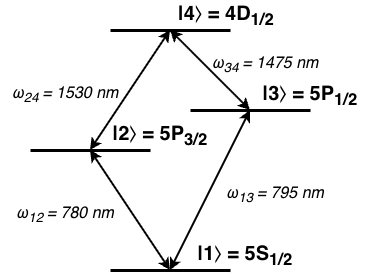
\includegraphics[width=\columnwidth]{Figs/DiamondAtom.png}
    \caption{A diamond configuration atomic system with  non-degenerate energy levels $\ket{1}, \ket{2}, \ket{3}, \ket{4}$ and respective energies $\hbar \omega_1$, $\hbar \omega_2$, $\hbar \omega_3$, and $\hbar \omega_4$. The system has allowed transitions $\ket{1} \leftrightarrow \ket{2}$, $\ket{1} \leftrightarrow \ket{3}$, $\ket{2} \leftrightarrow \ket{4}$, and $\ket{3} \leftrightarrow \ket{4}$}
    \label{DiamondAtom}
  \end{subfigure}
  \hfill
  \begin{subfigure}{0.45\textwidth}
    \centering
    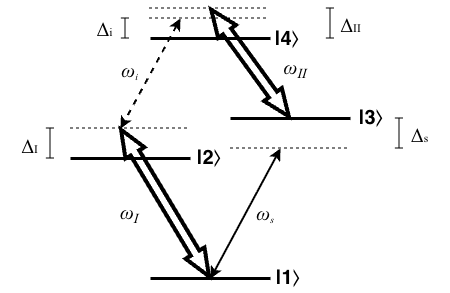
\includegraphics[width=\columnwidth]{Figs/DrivenDiamondAtom.png}
    \caption{A strong pump drives transition $\ket{1} \leftrightarrow \ket{2}$ at frequency $\omega_I$ with detuning $\Delta_I = \omega_I - \omega_{12}$, a separate strong pump drives transition $\ket{3} \leftrightarrow \ket{4}$ with detuning $\Delta_{II} = \omega_{II} - \omega_{34}$, a weak signal beam drives transition $\ket{1} \leftrightarrow \ket{3}$ with detuning $\Delta_{s} = \omega_{s} - \omega_{13}$, and a weak idler beam drives transition $\ket{2} \leftrightarrow \ket{4}$ with detuning $\Delta_{i} = \omega_{i} - \omega_{24}$.}
    \label{DrivenDiamondAtom}
  \end{subfigure}
  \caption{Diamond configuration atom diagrams.}
  \label{fig:twosidebyside}
\end{figure}

These states can be described without any interactions by the simple Hamiltonian

\begin{align}
    \hat{H}_0 &= \hbar \omega_1 \hat{\sigma}_{11} + \hbar \omega_2 \hat{\sigma}_{22} + \hbar \omega_3 \hat{\sigma}_{33} + \hbar \omega_4 \hat{\sigma}_{44}\\
    &= \hbar \left(\begin{array}{cccc}
        \omega_1 & 0 & 0 & 0\\
        0 & \omega_2 & 0 & 0\\
        0 & 0 & \omega_3 & 0\\
        0 & 0 & 0 & \omega_4\\
    \end{array}\right)
\end{align}


The reason we are attempting to obtain optical squeezing in the up-converted idler field is to transmit quantum information at telecom wavelengths. Therefore, we care about the quantized fields of the signal (input carrier of quantum information) and idler (output of frequency-converted quantum information) beams. Apply the theoretical resonant cavity approximation such that we consider photons in the Fock bases of the exact frequencies of the signal and idler beams to obtain the Hamiltonian

\begin{equation}
    \hat{H}_{photon} = \hbar \omega_{13} \hat{a}^{\dagger} \hat{a} + \hbar \omega_{24} \hat{b}^{\dagger} \hat{b}
\end{equation}

We then have the Hamiltonian describing these separate systems as


\begin{align}
    \hat{H}_S &= \hat{H}_0 + \hat{H}_{photon}\\
    &= \hbar \omega_1 \hat{\sigma}_{11} + \hbar \omega_2 \hat{\sigma}_{22} + \hbar \omega_3 \hat{\sigma}_{33} + \hbar \omega_4 \hat{\sigma}_{44}\nonumber \\
    &\;\;\;\;+ \hbar \omega_{13} \hat{a}^{\dagger} \hat{a} + \hbar \omega_{24} \hat{b}^{\dagger} \hat{b}
\end{align}


Each transition is driven by a laser as depicted in Fig.~\ref{DrivenDiamondAtom}. These driving fields cause significant coupling between states, requiring the definition of an interaction Hamiltonian. Under the dipole approximation following the procedure used in~\cite{QuantumInternet}, this interaction Hamiltonian takes the form  \textcolor{red}{NOTE - We do things slightly different than in the Du paper. They assume the dipole elements are all real-valued and swap $\sigma_{ij} \leftrightarrow \sigma_{ji}$ without swapping phases. This does not make any sense to me and seems like a hack or a mistake. We do not do this and end up with the addition of frequencies rather than detunings for the diagonal entries. I feel more confident with this because their method }

\subsection{Quantized Field Approach (Du's Procedure)}

\begin{equation}
    \hat{H}_{Int} = - \hat{\mathbf{d}} \cdot \mathbf{E}
\end{equation}
\begin{equation}
    \hat{\mathbf{d}} = \vec{d}_{12} \hat{\sigma}_{12} + \vec{d}_{13} \hat{\sigma}_{13} + \vec{d}_{24} \hat{\sigma}_{24} + \vec{d}_{34} \hat{\sigma}_{34} + h.c.
\end{equation}
\begin{equation}
    \mathbf{E} = \vec{E}_{I} + \vec{E}_{s} + \vec{E}_{i} + \vec{E}_{II}
\end{equation}
where $\vec{d}_{ij}$ is the dipole operator between states $i$ and $j$, the strong pump fields $\vec{E}_I$ and $\vec{E}_{II}$ are treated as classical fields, and the weak fields $\vec{E}_{s}$ and $\vec{E}_{i}$ are treated as quantized fields. Each field can be separated into a rapidly oscillating component and a slowly-varying envelope $\vec{\varepsilon}(t)$ as

\begin{align}
    \vec{E}_{I} &= \vec{\varepsilon}_I(t) e^{-i \omega_I t + i \vec{k}_I \cdot \vec{r}} + c.c.\\
    \vec{E}_{s} &= \vec{\varepsilon}_{s}(t) \hat{a} e^{i \vec{k}_{s} \cdot \vec{r}} + h.c.\\
    \vec{E}_{i} &= \vec{\varepsilon}_{i}(t) \hat{b} e^{i \vec{k}_{i} \cdot \vec{r}} + h.c.\\
    \vec{E}_{II} &= \vec{\varepsilon}_{II}(t) e^{-i \omega_{II} t + i \vec{k}_{II} \cdot \vec{r}} + c.c.\\
\end{align}
where $\hat{a}$ is the annihilation operator for the signal field, $\hat{b}$ is that of the idler field, $\vec{k}_j$ is the wavevector for each plane wave, and $\vec{r}$ is the position at which the field is experienced by the atom. 

\subsubsection{Classical Field Simplification via Rotating Wave Approximation}

Consider some coupled classical electric field $\vec{E}_c$ and dipole operator $\hat{\vec{d}}$
\begin{align}
    &\vec{E}_c = \vec{\varepsilon} (e^{i\phi} + e^{-i\phi}),\;\;\;\;\;\;\phi = kz - \omega t
\end{align}
\begin{align}
    &\hat{\vec{d}} = \vec{d}_{ij} \hat{\sigma}_{ij} + \vec{d}_{ji} \hat{\sigma}_{ji}
\end{align}
where we may arbitrarily take $\vec{\varepsilon} = \vec{\varepsilon}^*$ and $\vec{d}_{ij} = \vec{d}_{ji}$ (real-valued vectors). We can then expand
\begin{align}
    \vec{E}_c \cdot \hat{\vec{d}} = \vec{\varepsilon} \cdot \vec{d}_{ij} \left(\hat{\sigma}_{ij} e^{i\phi} + \hat{\sigma}_{ij} e^{-i\phi} + \hat{\sigma}_{ji} e^{i\phi} + \hat{\sigma}_{ji} e^{-i\phi}\right)
\end{align}

Go to the interaction picture where we have transition operators evolve as
\begin{align}
    \hat{\sigma}_{ij}(t) &= \hat{\sigma}_{ij} e^{-i \omega_0 t}\\
    \hat{\sigma}_{ji}(t) &= \hat{\sigma}_{ji} e^{i \omega_0 t}
\end{align}
where $\omega_0$ is the atomic transition frequency. We then have
\begin{align*}
    \vec{E}_c \cdot \hat{\vec{d}} = \vec{\varepsilon} \cdot \vec{d}_{ij} \left(
        \hat{\sigma}_{ij} e^{-i \omega_0 t} e^{i\phi} +
        \hat{\sigma}_{ij} e^{-i \omega_0 } e^{-i\phi} +
        \hat{\sigma}_{ji} e^{i \omega_0 t} e^{i\phi} +
        \hat{\sigma}_{ji} e^{i \omega_0 t} e^{-i\phi}
    \right)
\end{align*}
\begin{align}
    \vec{E}_c \cdot \hat{\vec{d}} = 
    \vec{\varepsilon} \cdot \vec{d}_{ij} \left(
        \hat{\sigma}_{ij}e^{i(kz - (\omega + \omega_0)t)} +
        \hat{\sigma}_{ij} e^{i(-kz + (\omega - \omega_0) t)} +
        \hat{\sigma}_{ji} e^{i(kz - (\omega - \omega_0) t)} +
        \hat{\sigma}_{ji} e^{i(-kz + (\omega + \omega_0) t)}
    \right)
\end{align}
Assuming that the driving field of frequency $\omega$ is near-resonant with the transition, we may apply the rotating wave approximation. Oscillations at frequency $\omega + \omega_0$ are so rapid in comparison to those at frequency $\omega - \omega_0$ that we may neglect them as they average to zero on optical timescales. Thus, we have

\begin{align}
    \vec{E}_c \cdot \hat{\vec{d}} \approx 
    \vec{\varepsilon} \cdot \vec{d}_{ij} \left(
        \hat{\sigma}_{ij} e^{i(-kz + (\omega - \omega_0) t)} +
        \hat{\sigma}_{ji} e^{i(kz - (\omega - \omega_0) t)}
    \right)
\end{align}
We may then go back to the Schr\"{o}dinger picture of state evolution and write
\begin{align}
    \vec{E}_c \cdot \hat{\vec{d}} \approx 
    \vec{\varepsilon} \cdot \vec{d}_{ij} \left(
        \hat{\sigma}_{ji} e^{i(kz - \omega t)} +
        \hat{\sigma}_{ij} e^{i(-kz + \omega t)}
    \right)
\end{align}

\subsubsection{Quantum Field Simplification via Rotating Wave Approximation}

Similar to the classical field approach, consider some coupled quantized electric field $\vec{E}_q$ and dipole operator $\hat{\vec{d}}$
\begin{align}
    \vec{E}_q \cdot \hat{\vec{d}} &=
    \vec{\varepsilon} \left(\hat{a} e^{i \vec{k} \cdot \vec{r}} + \hat{a}^{\dagger} e^{-i \vec{k} \cdot \vec{r}}\right) \cdot \left(\vec{d}_{ij} \hat{\sigma}_{ij} + \vec{d}_{ji} \hat{\sigma}_{ji}\right) \\
    &=
    \vec{\varepsilon} \cdot \vec{d}_{ij}\left(
        \hat{a} \hat{\sigma}_{ij} e^{i \vec{k} \cdot \vec{r}} +
        \hat{a}^{\dagger} \hat{\sigma}_{ij} e^{-i \vec{k} \cdot \vec{r}} +
        \hat{a} \vec{\sigma}_{ji} e^{i \vec{k} \cdot \vec{r}} +
        \hat{a}^{\dagger} \vec{\sigma}_{ji} e^{-i \vec{k} \cdot \vec{r}}
    \right)
\end{align}
We again go to the interaction picture in which we have operators evolve as
\begin{align}
    &\hat{a}(t) = \hat{a} e^{-i \omega t}\\
    &\hat{a}^{\dagger}(t) = \hat{a}^{\dagger} e^{i \omega t}\\
    &\hat{\sigma}_{ij}(t) = \hat{\sigma}_{ij} e^{-i \omega_0 t}\\
    &\hat{\sigma}_{ji}(t) = \hat{\sigma}_{ji} e^{i \omega_0 t}
\end{align}
So we have
\begin{align}
    \vec{E}_q \cdot \hat{\vec{d}} &=
    \vec{\varepsilon} \cdot \vec{d}_{ij}\left(
        \hat{a} e^{-i \omega t} e^{-i \omega_0 t} \hat{\sigma}_{ij} e^{i \vec{k} \cdot \vec{r}} +
        \hat{a}^{\dagger} e^{i \omega t} e^{-i \omega_0 t} \hat{\sigma}_{ij} e^{-i \vec{k} \cdot \vec{r}} +
        \hat{a} e^{-i \omega t} e^{i \omega_0 t}\vec{\sigma}_{ji} e^{i \vec{k} \cdot \vec{r}} +
        \hat{a}^{\dagger} e^{i \omega t} e^{i \omega_0 t}\vec{\sigma}_{ji} e^{-i \vec{k} \cdot \vec{r}}
    \right) \nonumber \\
    &=
    \vec{\varepsilon} \cdot \vec{d}_{ij}\left(
        \hat{a} e^{-i (\omega + \omega_0) t} \hat{\sigma}_{ij} e^{i \vec{k} \cdot \vec{r}} +
        \hat{a}^{\dagger} e^{-i (\omega - \omega_0) t} \hat{\sigma}_{ij} e^{-i \vec{k} \cdot \vec{r}} +
        \hat{a} e^{-i (\omega - \omega_0) t}\vec{\sigma}_{ji} e^{i \vec{k} \cdot \vec{r}} +
        \hat{a}^{\dagger} e^{i (\omega +\omega_0) t}\vec{\sigma}_{ji} e^{-i \vec{k} \cdot \vec{r}}
    \right) \nonumber \\
\end{align}
Then again by the rotating wave approximation we have
\begin{align}
    \vec{E}_q \cdot \hat{\vec{d}} &=
    \vec{\varepsilon} \cdot \vec{d}_{ij}\left(
        \hat{a}^{\dagger} e^{-i (\omega - \omega_0) t} \hat{\sigma}_{ij} e^{-i \vec{k} \cdot \vec{r}} +
        \hat{a} e^{-i (\omega - \omega_0) t}\vec{\sigma}_{ji} e^{i \vec{k} \cdot \vec{r}}
    \right) \nonumber \\
\end{align}
Going back to Schr\"{o}dinger picture then yields
\begin{align}
    \vec{E}_q \cdot \hat{\vec{d}} &=
    \vec{\varepsilon} \cdot \vec{d}_{ij}\left(
        \hat{a}^{\dagger} \hat{\sigma}_{ij} e^{-i \vec{k} \cdot \vec{r}} +
        \hat{a} \vec{\sigma}_{ji} e^{i \vec{k} \cdot \vec{r}}
    \right) \\
\end{align}

\subsubsection{Hamiltonian Expression}

Putting this all together, we obtain our interaction Hamiltonian as
\begin{align}
    \hat{H}_{Int} = &\left(\vec{d}_{12} \cdot \vec{\varepsilon}_I(t) \hat{\sigma}_{12} e^{-i \omega_I t + i \vec{k}_I \cdot \vec{r}} + c.c.\right)\nonumber \\
    &+ \left(\vec{d}_{13} \cdot \vec{\varepsilon}_{s}(t) \hat{\sigma}_{13} \hat{a}^{\dagger} e^{i \vec{k}_{s} \cdot \vec{r}} + h.c.\right)\nonumber \\
    &+ \left(\vec{d}_{24} \cdot \vec{\varepsilon}_{i}(t) \hat{\sigma}_{24} \hat{b}^{\dagger} e^{i \vec{k}_{i} \cdot \vec{r}} + h.c.\right)\nonumber \\
    &+ \left(\vec{d}_{34} \cdot \vec{\varepsilon}_{II}(t) \hat{\sigma}_{34} e^{-i \omega_{II} t + i \vec{k}_{II} \cdot \vec{r}} + c.c.\right)
\end{align}
The Rabi frequency (scaled by a factor of 2 here for simplicity) is the rate at which probability amplitudes between states oscillates in the presence of an electromagnetic field \cite{TODO} and is defined as

\begin{equation}
    \Omega = \frac{\vec{d} \cdot \vec{\varepsilon}}{\hbar}
\end{equation}
so we have \textcolor{red}{TODO - Quantum internet paper has $g$ instead of $\Omega$ for weak field-atom coupling. Should we have this instead?}
\begin{align}
    \hat{H}_{Int} = &\left(\hbar \Omega_{I}(t) \hat{\sigma}_{12} e^{i \omega_I t - i \vec{k}_I \cdot \vec{r}} + c.c.\right)\nonumber \\
    &+ \left(\hbar \Omega_{s}(t) \hat{\sigma}_{13} \hat{a}^{\dagger} e^{-i \vec{k}_{s} \cdot \vec{r}} + h.c.\right)\nonumber \\
    &+ \left(\hbar \Omega_{i}(t) \hat{\sigma}_{24} \hat{b}^{\dagger} e^{-i \vec{k}_{i} \cdot \vec{r}} + h.c.\right)\nonumber \\
    &+ \left(\hbar \Omega_{II}(t) \hat{\sigma}_{34} e^{i \omega_{II} t - i \vec{k}_{II} \cdot \vec{r}} + c.c.\right)
\end{align}
where we can notice the utility of the slowly-varying envelop approximation as the Rabi oscillations change on the timescale of the envelope rather than the rapidly oscillating carrier field. This is analogous to the logic of the rotating wave approximation where the carrier field oscillates so rapidly that we can take its average effect on the dipole to be zero. This allows us to approximately separate the Rabi frequencies from the field frequencies in the above. \textcolor{red}{TODO - Check this line of reasoning with MacRae}.

Combining this with $\hat{H}_S$ we obtain a Hamiltonian coupling atomic states with the weak signal and idler fields as

\begin{align}
    \hat{H} &= \hat{H}_S + \hat{H}_{Int}\\
    &= \hbar \omega_1 \hat{\sigma}_{11} + \hbar \omega_2 \hat{\sigma}_{22} + \hbar \omega_3 \hat{\sigma}_{33} + \hbar \omega_4 \hat{\sigma}_{44}\nonumber \\
    &\;\;\;\;+ \hbar \omega_{13} \hat{a}^{\dagger} \hat{a} + \hbar \omega_{24} \hat{b}^{\dagger} \hat{b}\nonumber \\
    &\;\;\;\;+ \left(\hbar \Omega_{I}(t) \hat{\sigma}_{12} e^{i \omega_I t - i \vec{k}_I \cdot \vec{r}} + c.c.\right)\nonumber \\
    &\;\;\;\;+ \left(\hbar \Omega_{s}(t) \hat{\sigma}_{13} \hat{a}^{\dagger} e^{-i \vec{k}_{s} \cdot \vec{r}} + h.c.\right)\nonumber \\
    &\;\;\;\;+ \left(\hbar \Omega_{i}(t) \hat{\sigma}_{24} \hat{b}^{\dagger} e^{-i \vec{k}_{i} \cdot \vec{r}} + h.c.\right)\nonumber \\
    &\;\;\;\;+ \left(\hbar \Omega_{II}(t) \hat{\sigma}_{34} e^{i \omega_{II} t - i \vec{k}_{II} \cdot \vec{r}} + c.c.\right)
\end{align}

Then define the unitary transformation which rotates with state $\ket{1}$ as reference

\begin{align}
    \hat{U}_{atom} &= \hat{\sigma}_{11} + e^{-i \omega_I t + i \vec{k}_I \cdot \vec{r}} \hat{\sigma}_{22} + e^{-i \omega_s t + i \vec{k}_s \cdot \vec{r}} \hat{\sigma}_{33} + e^{-i(\omega_{II} + \omega_s) t + i(\vec{k}_{II} + \vec{k}_s) \cdot \vec{r}} \hat{\sigma}_{44}
\end{align}
and the unitary transform rotating at the driving field frequencies which acts on the Fock photon bases

\begin{equation}
    \hat{U}_{photon} = e^{-i(\omega_s \hat{a}^{\dagger} \hat{a} + \omega_i \hat{b}^{\dagger} \hat{b})t}
\end{equation}
we then have the total unitary transformation of the coupled system as
\begin{equation}
    \hat{U} = \hat{U}_{atom} \otimes \hat{U}_{photon} =
    \left(
        \hat{\sigma}_{11} +
        e^{-i \omega_I t + i \vec{k}_I \cdot \vec{r}} \hat{\sigma}_{22} +
        e^{-i \omega_s t + i \vec{k}_s \cdot \vec{r}} \hat{\sigma}_{33} +
        e^{-i(\omega_{II} + \omega_s) t + i(\vec{k}_{II} + \vec{k}_s) \cdot \vec{r}} \hat{\sigma}_{44}
    \right)
    \otimes e^{-i(\omega_s \hat{a}^{\dagger} \hat{a} + \omega_i \hat{b}^{\dagger} \hat{b})t}.
\end{equation}
The total Hamiltonian can then be unitarily transformed as

\begin{equation}
    \tilde{H} = \hat{U}^{\dagger} \hat{H} \hat{U} + i \hbar (\partial_t \hat{U}^{\dagger}) \hat{U}.
\end{equation}
Since the bases are independent in this transformation, we may compute the corresponding components independently

\begin{equation}
    \hat{U}_{atom} = \left(\begin{array}{cccc}
        1 & 0 & 0 & 0\\
        0 & e^{-i \omega_I t + i \vec{k}_I \cdot \vec{r}} & 0 & 0\\
        0 & 0 & e^{-i \omega_s t + i \vec{k}_s \cdot \vec{r}} & 0\\
        0 & 0 & 0 & e^{-i(\omega_{II} + \omega_s) t + i(\vec{k}_{II} + \vec{k}_s) \cdot \vec{r}}\\
    \end{array}\right)
\end{equation}
\begin{align}
    \partial_t \hat{U}_{atom}^{\dagger}
    &=
    \partial_t \left(\begin{array}{cccc}
        1 & 0 & 0 & 0\\
        0 & e^{i \omega_I t - i \vec{k}_I \cdot \vec{r}} & 0 & 0\\
        0 & 0 & e^{i \omega_s t - i \vec{k}_s \cdot \vec{r}} & 0\\
        0 & 0 & 0 & e^{i(\omega_{II} + \omega_s) t - i(\vec{k}_{II} + \vec{k}_s) \cdot \vec{r}}\\
    \end{array}\right) \nonumber \\
    &=
    \left(\begin{array}{cccc}
        0 & 0 & 0 & 0\\
        0 & i \omega_I U_{22}^{*} & 0 & 0\\
        0 & 0 & i \omega_s U_{33}^{*} & 0\\
        0 & 0 & 0 & i(\omega_{II} + \omega_s)U_{44}^{*}\\
    \end{array}\right) \nonumber
\end{align}
\begin{align}
    i \hbar (\partial_t \hat{U}_{atom}^{\dagger}) \hat{U}_{atom}
    &=
    i \hbar \left(\begin{array}{cccc}
        0 & 0 & 0 & 0\\
        0 & i \omega_I U_{22}^{*} U_{22} & 0 & 0\\
        0 & 0 & i \omega_s U_{33}^{*} U_{33} & 0\\
        0 & 0 & 0 & i(\omega_{II} + \omega_s)U_{44}^{*} U_{44}\\
    \end{array}\right) \nonumber\\
    &=
    \hbar \left(\begin{array}{cccc}
        0 & 0 & 0 & 0\\
        0 & -\omega_I & 0 & 0\\
        0 & 0 & -\omega_s & 0\\
        0 & 0 & 0 & -(\omega_{II} + \omega_s)
    \end{array}\right)\nonumber\\
    &=
    -\hbar \omega_I \hat{\sigma}_{22} - \hbar \omega_s \hat{\sigma}_{33} - \hbar (\omega_{II} + \omega_s) \hat{\sigma}_{44}
\end{align}

\begin{equation}
    \partial_t \hat{U}_{photon}^{\dagger} =
    i(\omega_s \hat{a}^{\dagger} \hat{a} +
    \omega_i \hat{b}^{\dagger} \hat{b}) e^{i(\omega_s \hat{a}^{\dagger} \hat{a} +
    \omega_i \hat{b}^{\dagger} \hat{b})t}\nonumber
\end{equation}

\begin{align}
    i \hbar (\partial_t \hat{U}_{photon}^{\dagger}) \hat{U}_{photon}
    &=
    i^2 \hbar (\omega_s \hat{a}^{\dagger} \hat{a} +
    \omega_i \hat{b}^{\dagger} \hat{b}) e^{i(\omega_s \hat{a}^{\dagger} \hat{a} +
    \omega_i \hat{b}^{\dagger} \hat{b})t} e^{-i(\omega_s \hat{a}^{\dagger} \hat{a} +
    \omega_i \hat{b}^{\dagger} \hat{b})t}\nonumber\\
    &=
    -\hbar (\omega_s \hat{a}^{\dagger} \hat{a} + \omega_i \hat{b}^{\dagger} \hat{b})
\end{align}

\begin{equation}
    i \hbar (\partial_t \hat{U}^{\dagger}) \hat{U} =
    -\hbar \omega_I \hat{\sigma}_{22} -
    \hbar \omega_s \hat{\sigma}_{33} -
    \hbar (\omega_{II} + \omega_s) \hat{\sigma}_{44} -
    \hbar \omega_s \hat{a}^{\dagger} \hat{a} -
    \hbar \omega_i \hat{b}^{\dagger} \hat{b}
\end{equation}
Then expanding the other term we have
\begin{align}
    \hat{U}^{\dagger} \hat{H} \hat{U}
    &=
    \left(\hat{\sigma}_{11} + e^{i \omega_I t - i \vec{k}_I \cdot \vec{r}} \hat{\sigma}_{22} + e^{i \omega_s t - i \vec{k}_s \cdot \vec{r}} \hat{\sigma}_{33} + e^{i(\omega_{II} + \omega_s) t - i(\vec{k}_{II} + \vec{k}_s) \cdot \vec{r}} \hat{\sigma}_{44}\right)
    \otimes e^{i(\omega_s \hat{a}^{\dagger} \hat{a} + \omega_i \hat{b}^{\dagger} \hat{b})t}\nonumber\\
    &\;\;\;\;\cdot\biggl[ \hbar \omega_1 \hat{\sigma}_{11} + \hbar \omega_2 \hat{\sigma}_{22} + \hbar \omega_3 \hat{\sigma}_{33} + \hbar \omega_4 \hat{\sigma}_{44}\nonumber \\
    &\;\;\;\;\;\;\;\;+ \hbar \omega_{13} \hat{a}^{\dagger} \hat{a} + \hbar \omega_{24} \hat{b}^{\dagger} \hat{b}\nonumber \\
    &\;\;\;\;\;\;\;\;+ \hbar \left(\Omega_{I}(t) \hat{\sigma}_{12} e^{i \omega_I t - i \vec{k}_I \cdot \vec{r}} + \Omega_{I}^*(t) \hat{\sigma}_{21} e^{-i \omega_I t + i \vec{k}_I \cdot \vec{r}}\right)\nonumber \\
    &\;\;\;\;\;\;\;\;+ \hbar \left(\Omega_{s}(t) \hat{\sigma}_{13} \hat{a}^{\dagger} e^{-i \vec{k}_{s} \cdot \vec{r}} + \Omega_{s}^*(t) \hat{\sigma}_{31} \hat{a} e^{i \vec{k}_{s} \cdot \vec{r}}\right)\nonumber \\
    &\;\;\;\;\;\;\;\;+ \hbar \left(\Omega_{i}(t) \hat{\sigma}_{24} \hat{b}^{\dagger} e^{-i \vec{k}_{i} \cdot \vec{r}} + \Omega_{i}^*(t) \hat{\sigma}_{42} \hat{b} e^{i \vec{k}_{i} \cdot \vec{r}}\right)\nonumber \\
    &\;\;\;\;\;\;\;\;+ \hbar \left(\Omega_{II}(t) \hat{\sigma}_{34} e^{i \omega_{II} t - i \vec{k}_{II} \cdot \vec{r}} + \Omega_{II}^*(t) \hat{\sigma}_{43} e^{-i \omega_{II} t + i \vec{k}_{II} \cdot \vec{r}}\right)\biggr] \nonumber\\
    &\;\;\;\; \cdot
    \left(\hat{\sigma}_{11} + e^{-i \omega_I t + i \vec{k}_I \cdot \vec{r}} \hat{\sigma}_{22} + e^{-i \omega_s t + i \vec{k}_s \cdot \vec{r}} \hat{\sigma}_{33} + e^{-i(\omega_{II} + \omega_s) t + i(\vec{k}_{II} + \vec{k}_s) \cdot \vec{r}} \hat{\sigma}_{44}\right)
    \otimes e^{-i(\omega_s \hat{a}^{\dagger} \hat{a} + \omega_i \hat{b}^{\dagger} \hat{b})t}
\end{align}

Since $\hat{U}_{atom}$ commutes with $\hat{U}_{photon}$, and $\hat{U}_{atom}$ commutes with $\hat{H}_{photon}$ such that
\begin{equation}
    \hat{U}_{atom}^{\dagger} \hat{H}_{photon} \hat{U}_{atom} = \hat{U}_{atom}^{\dagger} \hat{U}_{atom} \hat{H}_{photon} = \hat{H}_{photon}
\end{equation}
we have

\begin{align}
    \frac{\hat{U}^{\dagger} \hat{H} \hat{U}}{\hbar}
    &= e^{i(\omega_s \hat{a}^{\dagger} \hat{a} + \omega_i \hat{b}^{\dagger} \hat{b})t} \nonumber \\
    &\;\;\;\;\otimes
    \left(\hat{\sigma}_{11} + e^{i \omega_I t - i \vec{k}_I \cdot \vec{r}} \hat{\sigma}_{22} + e^{i \omega_s t - i \vec{k}_s \cdot \vec{r}} \hat{\sigma}_{33} + e^{i(\omega_{II} + \omega_s) t - i(\vec{k}_{II} + \vec{k}_s) \cdot \vec{r}} \hat{\sigma}_{44}\right) \nonumber\\
    &\;\;\;\;\cdot\biggl[
        \omega_1 \hat{\sigma}_{11} + \omega_2 \hat{\sigma}_{22} + \omega_3 \hat{\sigma}_{33} + \omega_4 \hat{\sigma}_{44}\nonumber \\
        &\;\;\;\;\;\;\;\;+ \omega_{13} \hat{a}^{\dagger} \hat{a} + \omega_{24} \hat{b}^{\dagger} \hat{b}\nonumber \\
        &\;\;\;\;\;\;\;\;+ \left(\Omega_{I}(t) \hat{\sigma}_{12} e^{i \omega_I t - i \vec{k}_I \cdot \vec{r}} + \Omega_{I}^*(t) \hat{\sigma}_{21} e^{-i \omega_I t + i \vec{k}_I \cdot \vec{r}}\right)\nonumber \\
        &\;\;\;\;\;\;\;\;+ \left(\Omega_{s}(t) \hat{\sigma}_{13} \hat{a}^{\dagger} e^{-i \vec{k}_{s} \cdot \vec{r}} + \Omega_{s}^*(t) \hat{\sigma}_{31} \hat{a} e^{i \vec{k}_{s} \cdot \vec{r}}\right)\nonumber \\
        &\;\;\;\;\;\;\;\;+ \left(\Omega_{i}(t) \hat{\sigma}_{24} \hat{b}^{\dagger} e^{-i \vec{k}_{i} \cdot \vec{r}} + \Omega_{i}^*(t) \hat{\sigma}_{42} \hat{b} e^{i \vec{k}_{i} \cdot \vec{r}}\right)\nonumber \\
        &\;\;\;\;\;\;\;\;+ \left(\Omega_{II}(t) \hat{\sigma}_{34} e^{i \omega_{II} t - i \vec{k}_{II} \cdot \vec{r}} + \Omega_{II}^*(t) \hat{\sigma}_{43} e^{-i \omega_{II} t + i \vec{k}_{II} \cdot \vec{r}}\right)
    \biggr] \nonumber\\
    &\;\;\;\; \cdot
    \left(\hat{\sigma}_{11} + e^{-i \omega_I t + i \vec{k}_I \cdot \vec{r}} \hat{\sigma}_{22} + e^{-i \omega_s t + i \vec{k}_s \cdot \vec{r}} \hat{\sigma}_{33} + e^{-i(\omega_{II} + \omega_s) t + i(\vec{k}_{II} + \vec{k}_s) \cdot \vec{r}} \hat{\sigma}_{44}\right) \nonumber \\
    &\;\;\;\;\otimes e^{-i(\omega_s \hat{a}^{\dagger} \hat{a} + \omega_i \hat{b}^{\dagger} \hat{b})t} \nonumber \\
    &\;\;\;\;+ e^{i(\omega_s \hat{a}^{\dagger} \hat{a} + \omega_i \hat{b}^{\dagger} \hat{b})t}
    \left(\omega_{13} \hat{a}^{\dagger} \hat{a} + \omega_{24} \hat{b}^{\dagger} \hat{b}\right)
    e^{-i(\omega_s \hat{a}^{\dagger} \hat{a} + \omega_i \hat{b}^{\dagger} \hat{b})t} \nonumber \\
\end{align}

Separate the terms as

\begin{align}
    \hat{A}
    &=
    \left(\hat{\sigma}_{11} + e^{i \omega_I t - i \vec{k}_I \cdot \vec{r}} \hat{\sigma}_{22} + e^{i \omega_s t - i \vec{k}_s \cdot \vec{r}} \hat{\sigma}_{33} + e^{i(\omega_{II} + \omega_s) t - i(\vec{k}_{II} + \vec{k}_s) \cdot \vec{r}} \hat{\sigma}_{44}\right) \nonumber\\
    &\;\;\;\;\cdot\biggl[
        \omega_1 \hat{\sigma}_{11} + \omega_2 \hat{\sigma}_{22} + \omega_3 \hat{\sigma}_{33} + \omega_4 \hat{\sigma}_{44}\nonumber \\
        &\;\;\;\;\;\;\;\;+ \omega_{13} \hat{a}^{\dagger} \hat{a} + \omega_{24} \hat{b}^{\dagger} \hat{b}\nonumber \\
        &\;\;\;\;\;\;\;\;+ \left(\Omega_{I}(t) \hat{\sigma}_{12} e^{i \omega_I t - i \vec{k}_I \cdot \vec{r}} + \Omega_{I}^*(t) \hat{\sigma}_{21} e^{-i \omega_I t + i \vec{k}_I \cdot \vec{r}}\right)\nonumber \\
        &\;\;\;\;\;\;\;\;+ \left(\Omega_{s}(t) \hat{\sigma}_{13} \hat{a}^{\dagger} e^{-i \vec{k}_{s} \cdot \vec{r}} + \Omega_{s}^*(t) \hat{\sigma}_{31} \hat{a} e^{i \vec{k}_{s} \cdot \vec{r}}\right)\nonumber \\
        &\;\;\;\;\;\;\;\;+ \left(\Omega_{i}(t) \hat{\sigma}_{24} \hat{b}^{\dagger} e^{-i \vec{k}_{i} \cdot \vec{r}} + \Omega_{i}^*(t) \hat{\sigma}_{42} \hat{b} e^{i \vec{k}_{i} \cdot \vec{r}}\right)\nonumber \\
        &\;\;\;\;\;\;\;\;+ \left(\Omega_{II}(t) \hat{\sigma}_{34} e^{i \omega_{II} t - i \vec{k}_{II} \cdot \vec{r}} + \Omega_{II}^*(t) \hat{\sigma}_{43} e^{-i \omega_{II} t + i \vec{k}_{II} \cdot \vec{r}}\right)
    \biggr] \nonumber\\
    &\;\;\;\; \cdot
    \left(\hat{\sigma}_{11} + e^{-i \omega_I t + i \vec{k}_I \cdot \vec{r}} \hat{\sigma}_{22} + e^{-i \omega_s t + i \vec{k}_s \cdot \vec{r}} \hat{\sigma}_{33} + e^{-i(\omega_{II} + \omega_s) t + i(\vec{k}_{II} + \vec{k}_s) \cdot \vec{r}} \hat{\sigma}_{44}\right)\\\nonumber\\
    \hat{B}
    &=
    e^{i(\omega_s \hat{a}^{\dagger} \hat{a} + \omega_i \hat{b}^{\dagger} \hat{b})t} \hat{A} e^{-i(\omega_s \hat{a}^{\dagger} \hat{a} + \omega_i \hat{b}^{\dagger} \hat{b})t} \label{Beq} \\\nonumber\\
    \hat{C}
    &=
    \left(e^{i(\omega_s \hat{a}^{\dagger} \hat{a} + \omega_i \hat{b}^{\dagger} \hat{b})t}\right) \left(\omega_{13} \hat{a}^{\dagger}\hat{a} + \omega_{24} \hat{b}^{\dagger}\hat{b}\right)\left(e^{-i(\omega_s \hat{a}^{\dagger} \hat{a} + \omega_i \hat{b}^{\dagger} \hat{b})t}\right) \label{Unsimplified_C_eq}
\end{align}
Let us compute $\hat{A}$ using the facts that
\begin{equation}
    \hat{\sigma}_{ij} \hat{\sigma}_{kl} = \hat{\sigma}_{il} \delta_{jk},
\end{equation}
\begin{equation}
    \hat{\sigma}_{ij} \hat{\sigma}_{jk} \hat{\sigma}_{kl} = \hat{\sigma}_{il},
\end{equation}
and
\begin{equation}
    [\hat{\sigma}_{ij}, \hat{a}] = [\hat{\sigma}_{ij}, \hat{a}^{\dagger}] = [\hat{\sigma}_{ij}, \hat{b}] = [\hat{\sigma}_{ij}, \hat{b}^{\dagger}] = 0.
\end{equation}

First notice that

\begin{align}
&\left(
    \hat{\sigma}_{11} +
    e^{i \omega_I t - i \vec{k}_I \cdot \vec{r}} \hat{\sigma}_{22} +
    e^{i \omega_s t - i \vec{k}_s \cdot \vec{r}} \hat{\sigma}_{33} +
    e^{i(\omega_{II} + \omega_s) t - i(\vec{k}_{II} + \vec{k}_s) \cdot \vec{r}} \hat{\sigma}_{44}
\right) \nonumber\\
&\cdot\biggl[
    \omega_1 \hat{\sigma}_{11} +
    \omega_2 \hat{\sigma}_{22} +
    \omega_3 \hat{\sigma}_{33} +
    \omega_4 \hat{\sigma}_{44}
\biggr] \nonumber \\
&\cdot\left(
    \hat{\sigma}_{11} +
    e^{-i \omega_I t + i \vec{k}_I \cdot \vec{r}} \hat{\sigma}_{22} +
    e^{-i \omega_s t + i \vec{k}_s \cdot \vec{r}} \hat{\sigma}_{33} +
    e^{-i(\omega_{II} + \omega_s) t + i(\vec{k}_{II} + \vec{k}_s) \cdot \vec{r}} \hat{\sigma}_{44}
\right)\\
&\;\;\;\;\;\;\; = 
\biggl[
    \omega_1 \hat{\sigma}_{11} +
    \omega_2 \hat{\sigma}_{22} +
    \omega_3 \hat{\sigma}_{33} +
    \omega_4 \hat{\sigma}_{44}
\biggr] \nonumber \\
\end{align}

So we have

\begin{align}
    \hat{A}
    &=
    \omega_1 \hat{\sigma}_{11} + \omega_2 \hat{\sigma}_{22} + \omega_3 \hat{\sigma}_{33} + \omega_4 \hat{\sigma}_{44} \nonumber \\
    &\;\;\;\;+ \left(\hat{\sigma}_{11} + e^{i \omega_I t - i \vec{k}_I \cdot \vec{r}} \hat{\sigma}_{22} + e^{i \omega_s t - i \vec{k}_s \cdot \vec{r}} \hat{\sigma}_{33} + e^{i(\omega_{II} + \omega_s) t - i(\vec{k}_{II} + \vec{k}_s) \cdot \vec{r}} \hat{\sigma}_{44}\right) \nonumber\\
    &\;\;\;\;\cdot \biggl[
        \left(\Omega_{I}(t) \hat{\sigma}_{12} e^{i \omega_I t - i \vec{k}_I \cdot \vec{r}} + \Omega_{I}^*(t) \hat{\sigma}_{21} e^{-i \omega_I t + i \vec{k}_I \cdot \vec{r}}\right)\nonumber \\
        &\;\;\;\;\;\;+ \left(\Omega_{s}(t) \hat{\sigma}_{13} \hat{a}^{\dagger} e^{-i \vec{k}_{s} \cdot \vec{r}} + \Omega_{s}^*(t) \hat{\sigma}_{31} \hat{a} e^{i \vec{k}_{s} \cdot \vec{r}}\right)\nonumber \\
        &\;\;\;\;\;\;+ \left(\Omega_{i}(t) \hat{\sigma}_{24} \hat{b}^{\dagger} e^{-i \vec{k}_{i} \cdot \vec{r}} + \Omega_{i}^*(t) \hat{\sigma}_{42} \hat{b} e^{i \vec{k}_{i} \cdot \vec{r}}\right)\nonumber \\
        &\;\;\;\;\;\;+ \left(\Omega_{II}(t) \hat{\sigma}_{34} e^{i \omega_{II} t - i \vec{k}_{II} \cdot \vec{r}} + \Omega_{II}^*(t) \hat{\sigma}_{43} e^{-i \omega_{II} t + i \vec{k}_{II} \cdot \vec{r}}\right)
    \biggr] \nonumber \\
    &\;\;\;\; \cdot \left(\hat{\sigma}_{11} + e^{-i \omega_I t + i \vec{k}_I \cdot \vec{r}} \hat{\sigma}_{22} + e^{-i \omega_s t + i \vec{k}_s \cdot \vec{r}} \hat{\sigma}_{33} + e^{-i(\omega_{II} + \omega_s) t + i(\vec{k}_{II} + \vec{k}_s) \cdot \vec{r}} \hat{\sigma}_{44}\right)\nonumber \\ \nonumber\\
    &=
    \omega_1 \hat{\sigma}_{11} + \omega_2 \hat{\sigma}_{22} + \omega_3 \hat{\sigma}_{33} + \omega_4 \hat{\sigma}_{44} \nonumber \\
    &\;\;\;\;+
    \left(
        \Omega_{I}(t) \hat{\sigma}_{11} \hat{\sigma}_{12} \hat{\sigma}_{22} e^{-i \omega_I t + i \vec{k}_I \cdot \vec{r}} e^{i \omega_I t - i \vec{k}_I \cdot \vec{r}} +
        \Omega_{I}^*(t) e^{i \omega_I t - i \vec{k}_I \cdot \vec{r}} \hat{\sigma}_{22} \hat{\sigma}_{21} \hat{\sigma}_{11} e^{-i \omega_I t + i \vec{k}_I \cdot \vec{r}}
    \right)\nonumber \\
    &\;\;\;\;+
    \left(
        \Omega_{s}(t) \hat{\sigma}_{11} \hat{\sigma}_{13} \hat{\sigma}_{33} e^{-i \omega_s t + i \vec{k}_s \cdot \vec{r}} \hat{a}^{\dagger} e^{-i \vec{k}_{s} \cdot \vec{r}} +
        \Omega_{s}^*(t) e^{i \omega_s t - i \vec{k}_s \cdot \vec{r}} \hat{\sigma}_{33} \hat{\sigma}_{31} \hat{\sigma}_{11} \hat{a} e^{i \vec{k}_{s} \cdot \vec{r}}
    \right)\nonumber \\
    &\;\;\;\;+
    \Bigl(
        \Omega_{i}(t) e^{i \omega_I t - i \vec{k}_I \cdot \vec{r}} \hat{\sigma}_{22} \hat{\sigma}_{24} \hat{\sigma}_{44} e^{-i(\omega_{II} + \omega_s) t + i(\vec{k}_{II} + \vec{k}_s) \cdot \vec{r}} \hat{b}^{\dagger} e^{-i \vec{k}_{i} \cdot \vec{r}} \nonumber \\
    &\;\;\;\;\;\;\;\;+
        \Omega_{i}^*(t) e^{i(\omega_{II} + \omega_s) t - i(\vec{k}_{II} + \vec{k}_s) \cdot \vec{r}} \hat{\sigma}_{44} \hat{\sigma}_{42} \hat{\sigma}_{22} e^{-i \omega_I t + i \vec{k}_I \cdot \vec{r}} \hat{b} e^{i \vec{k}_{i} \cdot \vec{r}}
    \Bigr)\nonumber \\
    &\;\;\;\;+
    \Bigl(
        \Omega_{II}(t) e^{i \omega_s t - i \vec{k}_s \cdot \vec{r}} \hat{\sigma}_{33} \hat{\sigma}_{34} \hat{\sigma}_{44} e^{-i(\omega_{II} + \omega_s) t + i(\vec{k}_{II} + \vec{k}_s) \cdot \vec{r}} e^{i \omega_{II} t - i \vec{k}_{II} \cdot \vec{r}} \nonumber \\
    &\;\;\;\;\;\;\;\;+
        \Omega_{II}^*(t) e^{i(\omega_{II} + \omega_s) t - i(\vec{k}_{II} + \vec{k}_s) \cdot \vec{r}} \hat{\sigma}_{44} \hat{\sigma}_{43} \hat{\sigma}_{33} e^{-i \omega_s t + i \vec{k}_s \cdot \vec{r}} e^{-i \omega_{II} t + i \vec{k}_{II} \cdot \vec{r}}
    \Bigr) \nonumber \\ \nonumber \\
    &=
    \omega_1 \hat{\sigma}_{11} + \omega_2 \hat{\sigma}_{22} + \omega_3 \hat{\sigma}_{33} + \omega_4 \hat{\sigma}_{44} \nonumber \\
    &\;\;\;\;+
    \left(
        \Omega_{I}(t) \hat{\sigma}_{12} +
        \Omega_{I}^*(t) \hat{\sigma}_{21}
    \right)\nonumber \\
    &\;\;\;\;+
    \left(
        \Omega_{s}(t) e^{-i \omega_s t} \hat{\sigma}_{13} \hat{a}^{\dagger} +
        \Omega_{s}^*(t) e^{i \omega_s t} \hat{\sigma}_{31} \hat{a}
    \right)\nonumber \\
    &\;\;\;\;+
    \left(
        \Omega_{i}(t) e^{i(\omega_I - \omega_{II} - \omega_s) t - i(\vec{k}_I + \vec{k}_{i} - \vec{k}_{II} - \vec{k}_s) \cdot \vec{r}} \hat{\sigma}_{24} \hat{b}^{\dagger} +
        \Omega_{i}^*(t) e^{-i(\omega_{II} + \omega_s - \omega_I) t + i(\vec{k}_I + \vec{k}_{i} - \vec{k}_{II} - \vec{k}_s) \cdot \vec{r}} \hat{\sigma}_{42} \hat{b}
    \right)\nonumber \\
    &\;\;\;\;+
    \left(
        \Omega_{II}(t) \hat{\sigma}_{34} +
        \Omega_{II}^*(t) \hat{\sigma}_{43}
    \right)
\end{align}
We can then impose the energy conservation condition and phase match condition (in that order as follows)
\begin{align}
    \omega_I + \omega_i &= \omega_s + \omega_{II}\\
    k_I + k_i &= k_s + k_{II}
\end{align}

\begin{align}
    \hat{A}
    &=
    \omega_1 \hat{\sigma}_{11} + \omega_2 \hat{\sigma}_{22} + \omega_3 \hat{\sigma}_{33} + \omega_4 \hat{\sigma}_{44} \nonumber \\
    &\;\;\;\;+
    \left(
        \Omega_{I}(t) \hat{\sigma}_{12} +
        \Omega_{I}^*(t) \hat{\sigma}_{21}
    \right)\nonumber \\
    &\;\;\;\;+
    \left(
        \Omega_{s}(t) e^{-i \omega_s t} \hat{\sigma}_{13} \hat{a}^{\dagger} +
        \Omega_{s}^*(t) e^{i \omega_s t} \hat{\sigma}_{31} \hat{a}
    \right)\nonumber \\
    &\;\;\;\;+
    \left(
        \Omega_{i}(t) e^{-i\omega_i t} \hat{\sigma}_{24} \hat{b}^{\dagger} +
        \Omega_{i}^*(t) e^{i\omega_i t} \hat{\sigma}_{42} \hat{b}
    \right)\nonumber \\
    &\;\;\;\;+
    \left(
        \Omega_{II}(t) \hat{\sigma}_{34} +
        \Omega_{II}^*(t) \hat{\sigma}_{43}
    \right)
\end{align}
Now we may compute $\hat{B}$ from eq.~\eqref{Beq} as
\begin{align}
    \hat{B}
    &=
    e^{i(\omega_s \hat{a}^{\dagger} \hat{a} + \omega_i \hat{b}^{\dagger} \hat{b})t}
    \hat{A}
    e^{-i(\omega_s \hat{a}^{\dagger} \hat{a} + \omega_i \hat{b}^{\dagger} \hat{b})t} \nonumber \\
    &=
    e^{i(\omega_s \hat{a}^{\dagger} \hat{a} + \omega_i \hat{b}^{\dagger} \hat{b})t} \nonumber\\
    &\;\;\;\;
    \cdot \biggl[
        \omega_1 \hat{\sigma}_{11} +
        \omega_2 \hat{\sigma}_{22} +
        \omega_3 \hat{\sigma}_{33} +
        \omega_4 \hat{\sigma}_{44} \nonumber \\
        &\;\;\;\;\;\;+
        \left(
            \Omega_{I}(t) \hat{\sigma}_{12} +
            \Omega_{I}^*(t) \hat{\sigma}_{21}
        \right)\nonumber \\
        &\;\;\;\;\;\;+
        \left(
            \Omega_{s}(t) e^{-i \omega_s t} \hat{\sigma}_{13} \hat{a}^{\dagger} +
            \Omega_{s}^*(t) e^{i \omega_s t} \hat{\sigma}_{31} \hat{a}
        \right)\nonumber \\
        &\;\;\;\;\;\;+
        \left(
            \Omega_{i}(t) e^{-i\omega_i t} \hat{\sigma}_{24} \hat{b}^{\dagger} +
            \Omega_{i}^*(t) e^{i\omega_i t} \hat{\sigma}_{42} \hat{b}
        \right)\nonumber \\
        &\;\;\;\;\;\;+
        \left(
            \Omega_{II}(t) \hat{\sigma}_{34} +
            \Omega_{II}^*(t) \hat{\sigma}_{43}
        \right)
    \biggr] \nonumber\\
    &\;\;\;\;\cdot
    e^{-i(\omega_s \hat{a}^{\dagger} \hat{a} + \omega_i \hat{b}^{\dagger} \hat{b})t}
\end{align}
which, via commutation relations, simplifies to 
\begin{align}\label{Unsimplified_B_eq}
    \hat{B}
    &=
    \omega_1 \hat{\sigma}_{11} +
    \omega_2 \hat{\sigma}_{22} +
    \omega_3 \hat{\sigma}_{33} +
    \omega_4 \hat{\sigma}_{44} \nonumber \\
    &\;\;\;\;\;\;+
    \left(
        \Omega_{I}(t) \hat{\sigma}_{12} +
        \Omega_{I}^*(t) \hat{\sigma}_{21}
    \right)\nonumber \\
    &\;\;\;\;\;\;+
    \left(
        \Omega_{II}(t) \hat{\sigma}_{34} +
        \Omega_{II}^*(t) \hat{\sigma}_{43}
    \right) \nonumber \\
    &\;\;\;\;\;\;+
    e^{i\omega_s \hat{a}^{\dagger} \hat{a}t}
    \left(
        \Omega_{s}(t) e^{-i \omega_s t} \hat{\sigma}_{13} \hat{a} +
        \Omega_{s}^*(t) e^{i \omega_s t} \hat{\sigma}_{31} \hat{a}^{\dagger}
    \right)
    e^{-i\omega_s \hat{a}^{\dagger} \hat{a}t}\nonumber \\
    &\;\;\;\;\;\;+
    e^{i \omega_i \hat{b}^{\dagger} \hat{b} t}
    \left(
        \Omega_{i}(t) e^{-i\omega_i t} \hat{\sigma}_{24} \hat{b} +
        \Omega_{i}^*(t) e^{i\omega_i t} \hat{\sigma}_{42} \hat{b}^{\dagger}
    \right) e^{-i \omega_i \hat{b}^{\dagger} \hat{b} t}
\end{align}
We must then compute
\begin{align}
    e^{i\omega_s \hat{a}^{\dagger} \hat{a}t} \hat{a} e^{-i\omega_s \hat{a}^{\dagger} \hat{a}t}
\end{align}
which we can do via the Baker-Campbell-Hausdorff formula
\begin{align}
    e^{\hat{X}} \hat{Y} e^{-\hat{X}} = \sum_{n=0}^{\infty} \frac{{[X, Y]}_n}{n!} = Y + [X, Y] + \frac{1}{2!}[X, [X, Y]] + \cdots
\end{align}
where
\begin{align}
    {[X, Y]}_n = \underbrace{[X, [X, \ldots, [X, [X}_{\text{n times}}, Y]], \ldots]]
\end{align}
\begin{align}
    e^{i\omega_s \hat{a}^{\dagger} \hat{a}t} \hat{a} e^{-i\omega_s \hat{a}^{\dagger} \hat{a}t} &= \sum_{n=0}^{\infty} \frac{{[i\omega_s \hat{a}^{\dagger} \hat{a}t, \hat{a}]}_n}{n!} \nonumber \\
    e^{i\omega_s \hat{a}^{\dagger} \hat{a}t} \hat{a} e^{-i\omega_s \hat{a}^{\dagger} \hat{a}t} &= \sum_{n=0}^{\infty} \frac{{[i\omega_s \hat{a}^{\dagger} \hat{a}t, \hat{a}]}_n}{n!} \nonumber \\
    &= \hat{a} + [i\omega_s \hat{a}^{\dagger} \hat{a}t, \hat{a}] + \frac{1}{2!}[i\omega_s \hat{a}^{\dagger} \hat{a}t, [i\omega_s \hat{a}^{\dagger} \hat{a}t, \hat{a}]] + \frac{1}{3!}[i\omega_s \hat{a}^{\dagger} \hat{a}t, [i\omega_s \hat{a}^{\dagger} \hat{a}t, [i\omega_s \hat{a}^{\dagger} \hat{a}t, \hat{a}]]] + \cdots \nonumber \\
    &= \hat{a} + i \omega_s t [\hat{a}^{\dagger} \hat{a}, \hat{a}] + \frac{(i \omega_s t)^2}{2!} [\hat{a}^{\dagger} \hat{a}, [\hat{a}^{\dagger} \hat{a}, \hat{a}]] + \frac{(i \omega_s t)^3}{3!}[\hat{a}^{\dagger} \hat{a}, [\hat{a}^{\dagger} \hat{a}, [\hat{a}^{\dagger} \hat{a}, \hat{a}]]] + \cdots
\end{align}
To move forward we must then compute the commutators
\begin{align}
    [\hat{a}^{\dagger} \hat{a}, \hat{a}] &=
    \hat{a}^{\dagger} \hat{a} \hat{a} - \hat{a} \hat{a}^{\dagger} \hat{a} \nonumber
\end{align}
use the commutation relation
\begin{align}
    [\hat{a}, \hat{a}^{\dagger}] = \hat{a} \hat{a}^{\dagger} - \hat{a}^{\dagger} \hat{a} = 1 \nonumber\\
    \hat{a} \hat{a}^{\dagger} = 1 + \hat{a}^{\dagger} \hat{a}
\end{align}
to obtain
\begin{align}
    [\hat{a}^{\dagger} \hat{a}, \hat{a}] &= \hat{a}^{\dagger} \hat{a} \hat{a} - (1 + \hat{a}^{\dagger} \hat{a}) \hat{a} \nonumber \\
    &= \hat{a}^{\dagger} \hat{a} \hat{a} - \hat{a} - \hat{a}^{\dagger} \hat{a}\hat{a} \nonumber \\
    &= - \hat{a}
\end{align}
Then we have that
\begin{align}
    [\hat{a}^{\dagger} \hat{a}, [\hat{a}^{\dagger} \hat{a}, \hat{a}]] &= [\hat{a}^{\dagger} \hat{a}, -\hat{a}] \nonumber \\
    &= -[\hat{a}^{\dagger} \hat{a}, \hat{a}] \nonumber \\
    &= \hat{a}
\end{align}
Assume this pattern holds until the $k^{th}$ application
\begin{equation}
    {[\hat{a}^{\dagger} \hat{a}, \hat{a}]}_{k} = {(-1)}^k \hat{a}\;\;\;\;\;\;\text{(Induction Hypothesis)}
\end{equation}
then consider the ${(k+1)}^{th}$ step
\begin{align}
    {[\hat{a}^{\dagger} \hat{a}, \hat{a}]}_{k+1} &= [\hat{a}^{\dagger} \hat{a}, {[\hat{a}^{\dagger} \hat{a}, \hat{a}]}_{k}] \nonumber \\
    &= [\hat{a}^{\dagger} \hat{a}, {(-1)}^k \hat{a}] \nonumber \\
    &= {(-1)}^k [\hat{a}^{\dagger} \hat{a}, \hat{a}] \nonumber \\
    &= {(-1)}^k (-\hat{a}) \nonumber \\
    &= {(-1)}^{k+1} \hat{a} \nonumber
\end{align}
Thus, by induction we have that
\begin{equation}
    {[\hat{a}^{\dagger} \hat{a}, \hat{a}]}_{n} = {(-1)}^{n} \hat{a}
\end{equation}
So we may write
\begin{align}
    e^{i\omega_s \hat{a}^{\dagger} \hat{a}t} \hat{a} e^{-i\omega_s \hat{a}^{\dagger} \hat{a}t}
    &= \hat{a} + i \omega_s t [\hat{a}^{\dagger} \hat{a}, \hat{a}] + \frac{(i \omega_s t)^2}{2!} [\hat{a}^{\dagger} \hat{a}, [\hat{a}^{\dagger} \hat{a}, \hat{a}]] + \frac{(i \omega_s t)^3}{3!}[\hat{a}^{\dagger} \hat{a}, [\hat{a}^{\dagger} \hat{a}, [\hat{a}^{\dagger} \hat{a}, \hat{a}]]] + \cdots \nonumber \\
    &= \hat{a} + i \omega_s t (-\hat{a}) + \frac{(i \omega_s t)^2}{2!} (\hat{a}) + \frac{(i \omega_s t)^3}{3!}(-\hat{a}) + \cdots \nonumber \\
    &= \hat{a}\left(1 - i \omega_s t + \frac{(i \omega_s t)^2}{2!} - \frac{(i \omega_s t)^3}{3!} + \cdots \right)\nonumber \\
    &= \hat{a}\left(1 + (-i \omega_s t) + \frac{(-i \omega_s t)^2}{2!} + \frac{(-i \omega_s t)^3}{3!} + \cdots \right)\nonumber \\
    &= \hat{a} \sum_{n=0}^{\infty} \frac{(-i \omega_s t)^n}{n!}\nonumber \\
    &= \hat{a} e^{-i \omega_s t}
\end{align}
Then we can find
\begin{align}
    &
    {(e^{i\omega_s \hat{a}^{\dagger} \hat{a}t} \hat{a} e^{-i\omega_s \hat{a}^{\dagger} \hat{a}t})}^{\dagger} =
    {(\hat{a} e^{-i \omega_s t})}^{\dagger} \nonumber \\
    &
    \left(e^{-i\omega_s \hat{a}^{\dagger} \hat{a}t}\right)^{\dagger} \hat{a}^{\dagger} \left(e^{i\omega_s \hat{a}^{\dagger} \hat{a}t}\right)^{\dagger} =
    \hat{a}^{\dagger} e^{i \omega_s t} \nonumber \\
    &
    e^{i\omega_s \left(\hat{a}^{\dagger} \hat{a}\right)^{\dagger}t} \hat{a}^{\dagger} e^{i\omega_s \left(\hat{a}^{\dagger} \hat{a}\right)^{\dagger}t} =
    \hat{a}^{\dagger} e^{i \omega_s t} \nonumber \\
    &
    e^{i\omega_s \hat{a}^{\dagger} \left(\hat{a}^{\dagger} \right)^{\dagger} t} \hat{a}^{\dagger} e^{i\omega_s \hat{a}^{\dagger} \left(\hat{a}^{\dagger} \right)^{\dagger} \hat{a} t} =
    \hat{a}^{\dagger} e^{i \omega_s t} \nonumber \\
    &
    e^{i\omega_s \hat{a}^{\dagger} \hat{a}t} \hat{a}^{\dagger} e^{-i\omega_s \hat{a}^{\dagger} \hat{a}t} =
    \hat{a}^{\dagger} e^{i \omega_s t}
\end{align}
Similarly
\begin{align}
    &e^{i\omega_i \hat{b}^{\dagger} \hat{b}t} \hat{b} e^{-i\omega_i \hat{b}^{\dagger} \hat{b}t} = \hat{b} e^{-i \omega_i t}\\
    &e^{i\omega_i \hat{b}^{\dagger} \hat{b}t} \hat{b}^{\dagger} e^{-i\omega_i \hat{b}^{\dagger} \hat{b}t} = \hat{b}^{\dagger} e^{i \omega_i t}
\end{align}
So we can simplify eq.~\eqref{Unsimplified_B_eq} to
\begin{align}
    \hat{B}
    &=
    \omega_1 \hat{\sigma}_{11} + \omega_2 \hat{\sigma}_{22} + \omega_3 \hat{\sigma}_{33} + \omega_4 \hat{\sigma}_{44} \nonumber \\
    &\;\;\;\;+
    \left(
        \Omega_{I}(t) \hat{\sigma}_{12} +
        \Omega_{I}^*(t) \hat{\sigma}_{21}
    \right)\nonumber \\
    &\;\;\;\;+
    \left(
        \Omega_{II}(t) \hat{\sigma}_{34} +
        \Omega_{II}^*(t) \hat{\sigma}_{43}
    \right) \nonumber \\
    &\;\;\;\;+
    \left(
        \Omega_{s}(t) e^{-i \omega_s t} \hat{\sigma}_{13} \hat{a}^{\dagger} e^{i \omega_s t} +
        \Omega_{s}^*(t) e^{i \omega_s t} \hat{\sigma}_{31} \hat{a} e^{-i \omega_s t}
    \right) \nonumber \\
    &\;\;\;\;+
    \left(
        \Omega_{i}(t) e^{-i\omega_i t} \hat{\sigma}_{24} \hat{b}^{\dagger} e^{i \omega_i t}
        + \Omega_{i}^*(t) e^{i\omega_i t} \hat{\sigma}_{42} \hat{b} e^{-i \omega_i t}
    \right)\nonumber
\end{align}

\begin{align}
    \hat{B}
    &=
    \omega_1 \hat{\sigma}_{11} + \omega_2 \hat{\sigma}_{22} + \omega_3 \hat{\sigma}_{33} + \omega_4 \hat{\sigma}_{44} \nonumber \\
    &\;\;\;\;+
    \left(
        \Omega_{I}(t) \hat{\sigma}_{12} +
        \Omega_{I}^*(t) \hat{\sigma}_{21}
    \right)\nonumber \\
    &\;\;\;\;+
    \left(
        \Omega_{s}(t) \hat{a}^{\dagger} \hat{\sigma}_{13} +
        \Omega_{s}^*(t) \hat{a} \hat{\sigma}_{31}
    \right) \nonumber \\
    &\;\;\;\;+
    \left(
        \Omega_{i}(t) \hat{b}^{\dagger} \hat{\sigma}_{24} +
        \Omega_{i}^*(t) \hat{b} \hat{\sigma}_{42}
    \right) \nonumber \\
    &\;\;\;\;+
    \left(
        \Omega_{II}(t) \hat{\sigma}_{34} +
        \Omega_{II}^*(t) \hat{\sigma}_{43}
    \right)
\end{align}

\begin{align}
    \hat{B} &= \left(\begin{array}{cccc}
        \omega_1  & \Omega_{I}(t) & \Omega_{s}(t) \hat{a}^{\dagger} & 0\\
        \Omega_{I}^*(t) & \omega_2  & 0 & \Omega_{i}(t) \hat{b}^{\dagger}\\
        \Omega_{s}^*(t) \hat{a} & 0 & \omega_3 & \Omega_{II}(t)\\
        0 & \Omega_{i}^*(t) \hat{b} & \Omega_{II}^*(t) & \omega_4
    \end{array}\right)
\end{align}

Now consider the next component from eq.~\eqref{Unsimplified_C_eq}
\begin{align}
    \hat{C} &= \left(e^{i(\omega_s \hat{a}^{\dagger} \hat{a} + \omega_i \hat{b}^{\dagger} \hat{b})t}\right) \left(\omega_{13} \hat{a}^{\dagger}\hat{a} + \omega_{24} \hat{b}^{\dagger}\hat{b}\right)\left(e^{-i(\omega_s \hat{a}^{\dagger} \hat{a} + \omega_i \hat{b}^{\dagger} \hat{b})t}\right) \nonumber \\
    &= \omega_{13} e^{i\omega_s \hat{a}^{\dagger} \hat{a}t} \hat{a}^{\dagger}\hat{a} e^{-i\omega_s \hat{a}^{\dagger} \hat{a}} + \omega_{24} e^{\omega_i \hat{b}^{\dagger} \hat{b}t} \hat{b}^{\dagger}\hat{b} e^{-\omega_i \hat{b}^{\dagger} \hat{b}t}
\end{align}
using the commutation relation for the distinct fields
\begin{equation}
    \left[ \hat{a}^{\dagger} \hat{a}, \hat{b}^{\dagger} \hat{b} \right] = 0
\end{equation}
Then we may expand the exponentials as
\begin{align}
    e^{i\omega \hat{a}^{\dagger} \hat{a} t} \hat{a}^{\dagger} \hat{a} e^{-i\omega \hat{a}^{\dagger} \hat{a} t}
    &= \left[\sum_{n=0}^{\infty} \frac{\left(i\omega \hat{a}^{\dagger} \hat{a} t\right)^n}{n!}\right] \hat{a}^{\dagger} \hat{a} \left[\sum_{n=0}^{\infty} \frac{\left(-i\omega \hat{a}^{\dagger} \hat{a} t\right)^n}{n!}\right] \nonumber \\
    &= \left[\sum_{n=0}^{\infty} \frac{\left(i \omega t\right)^n \left(\hat{a}^{\dagger} \hat{a}\right)^{n+1}}{n!}\right] \left[\sum_{n=0}^{\infty} \frac{\left(-i\omega \hat{a}^{\dagger} \hat{a} t\right)^n}{n!}\right] \nonumber \\
    &= \hat{a}^{\dagger} \hat{a} \left[\sum_{n=0}^{\infty} \frac{\left(i\omega \hat{a}^{\dagger} \hat{a} t\right)^n}{n!}\right] \left[\sum_{n=0}^{\infty} \frac{\left(-i\omega \hat{a}^{\dagger} \hat{a} t\right)^n}{n!}\right] \nonumber \\
    &= \hat{a}^{\dagger} \hat{a} e^{i\omega \hat{a}^{\dagger} \hat{a} t}  e^{-i\omega \hat{a}^{\dagger} \hat{a} t} \nonumber \\
    &= \hat{a}^{\dagger} \hat{a}
\end{align}
which follows similarly for
\begin{equation}
    e^{i\omega \hat{b}^{\dagger} \hat{b} t} \hat{b}^{\dagger} \hat{b} e^{-i\omega \hat{b}^{\dagger} \hat{b} t} = \hat{b}^{\dagger} \hat{b}
\end{equation}
yielding
\begin{equation}
    \hat{C} = \omega_{13} \hat{a}^{\dagger}\hat{a} + \omega_{24} \hat{b}^{\dagger}\hat{b}
\end{equation}
Thus, we have
\begin{align}
    \frac{\hat{U}^{\dagger} \hat{H} \hat{U}}{\hbar}
    &=
    \hat{B} + \hat{C} \nonumber\\
    &=
    \omega_1 \hat{\sigma}_{11} + \omega_2 \hat{\sigma}_{22} + \omega_3 \hat{\sigma}_{33} + \omega_4 \hat{\sigma}_{44} \nonumber \\
    &\;\;\;\;+
    \left(
        \Omega_{I}(t) \hat{\sigma}_{12} +
        \Omega_{I}^*(t) \hat{\sigma}_{21}
    \right)\nonumber \\
    &\;\;\;\;+
    \left(
        \Omega_{s}(t) \hat{a}^{\dagger} \hat{\sigma}_{13} +
        \Omega_{s}^*(t) \hat{a} \hat{\sigma}_{31}
    \right) \nonumber \\
    &\;\;\;\;+
    \left(
        \Omega_{i}(t) \hat{b}^{\dagger} \hat{\sigma}_{24} +
        \Omega_{i}^*(t) \hat{b} \hat{\sigma}_{42}
    \right) \nonumber \\
    &\;\;\;\;+
    \left(
        \Omega_{II}(t) \hat{\sigma}_{34}
        + \Omega_{II}^*(t) \hat{\sigma}_{43}
    \right) \nonumber \\
    &\;\;\;\;+
    \omega_{13} \hat{a}^{\dagger}\hat{a} +
    \omega_{24} \hat{b}^{\dagger}\hat{b}
\end{align}
Then we have the unitary transformation as
\begin{align}
    \tilde{H}
    &=
    \hat{U}^{\dagger} \hat{H} \hat{U} + i \hbar (\partial_t \hat{U}^{\dagger}) \hat{U} \nonumber \\
    &=
    \hbar \biggl[
        \omega_1 \hat{\sigma}_{11} +
        \omega_2 \hat{\sigma}_{22} +
        \omega_3 \hat{\sigma}_{33} +
        \omega_4 \hat{\sigma}_{44} \nonumber \\
        &\;\;\;\;\;\;+
        \left(
            \Omega_{I}(t) \hat{\sigma}_{12} +
            \Omega_{I}^*(t) \hat{\sigma}_{21}
        \right)\nonumber \\
        &\;\;\;\;\;\;+
        \left(
            \Omega_{s}(t) \hat{a}^{\dagger} \hat{\sigma}_{13} +
            \Omega_{s}^*(t) \hat{a} \hat{\sigma}_{31}
        \right) \nonumber \\
        &\;\;\;\;\;\;+
        \left(
            \Omega_{i}(t) \hat{b}^{\dagger} \hat{\sigma}_{24} +
            \Omega_{i}^*(t) \hat{b} \hat{\sigma}_{42}
        \right) \nonumber \\
        &\;\;\;\;\;\;+
        \left(
            \Omega_{II}(t) \hat{\sigma}_{34} +
            \Omega_{II}^*(t) \hat{\sigma}_{43}
        \right) \nonumber \\
        &\;\;\;\;\;\;+
        \omega_{13} \hat{a}^{\dagger}\hat{a} +
        \omega_{24} \hat{b}^{\dagger}\hat{b}
    \biggr]\nonumber \\
    &\;\;\;\;+
    \hbar \biggl[
        -\omega_I \hat{\sigma}_{22} -
        \omega_s \hat{\sigma}_{33} -
        (\omega_{II} + \omega_s) \hat{\sigma}_{44} -
        \omega_s \hat{a}^{\dagger} \hat{a} -
        \omega_i \hat{b}^{\dagger} \hat{b}
    \biggr] \nonumber
\end{align}
\begin{align}
    \tilde{H}
    &=
    \hbar \biggl[
        \omega_1 \hat{\sigma}_{11} +
        (\omega_2 - \omega_I) \hat{\sigma}_{22} +
        (\omega_3 - \omega_s) \hat{\sigma}_{33} +
        (\omega_4 - \omega_{II} + \omega_s) \hat{\sigma}_{44} \nonumber \\
        &\;\;\;\;+
        \left(
            \Omega_{I}(t) \hat{\sigma}_{12} +
            \Omega_{I}^*(t) \hat{\sigma}_{21}
        \right)\nonumber \\
        &\;\;\;\;+
        \left(
            \Omega_{s}(t) \hat{a}^{\dagger} \hat{\sigma}_{13} +
            \Omega_{s}^*(t) \hat{a} \hat{\sigma}_{31}
        \right) \nonumber \\
        &\;\;\;\;+ 
        \left(
            \Omega_{i}(t) \hat{b}^{\dagger} \hat{\sigma}_{24} +
            \Omega_{i}^*(t) \hat{b} \hat{\sigma}_{42}
        \right) \nonumber \\
        &\;\;\;\;+
        \left(
            \Omega_{II}(t) \hat{\sigma}_{34} +
            \Omega_{II}^*(t) \hat{\sigma}_{43}
        \right) \nonumber \\
        &\;\;\;\;+
        (\omega_{13} - \omega_s) \hat{a}^{\dagger}\hat{a} +
        (\omega_{24} - \omega_i) \hat{b}^{\dagger}\hat{b}
    \biggr]
\end{align}

We can then choose to arbitrarily shift the energy levels of the Hamiltonian by
\begin{align}
    \tilde{H}
    &\rightarrow
    \tilde{H} - \hbar \omega_1 \hat{\mathbbm{1}} \nonumber \\
    &\rightarrow
    \hbar \biggl[
        (\omega_2 - \omega_1 - \omega_I) \hat{\sigma}_{22} +
        (\omega_3 - \omega_1 - \omega_s) \hat{\sigma}_{33} +
        (\omega_4 - \omega_1 - \omega_{II} - \omega_s) \hat{\sigma}_{44} \nonumber \\
        &\;\;\;\;+
        \left(
            \Omega_{I}(t) \hat{\sigma}_{12} +
            \Omega_{I}^*(t) \hat{\sigma}_{21}
        \right)\nonumber \\
        &\;\;\;\;+
        \left(
            \Omega_{s}(t) \hat{a}^{\dagger} \hat{\sigma}_{13} +
            \Omega_{s}^*(t) \hat{a} \hat{\sigma}_{31}
        \right) \nonumber \\
        &\;\;\;\;+
        \left(
            \Omega_{i}(t) \hat{b}^{\dagger} \hat{\sigma}_{24} +
            \Omega_{i}^*(t) \hat{b} \hat{\sigma}_{42}
        \right) \nonumber \\
        &\;\;\;\;+
        \left(
            \Omega_{II}(t) \hat{\sigma}_{34} +
            \Omega_{II}^*(t) \hat{\sigma}_{43}
        \right) \nonumber \\
        &\;\;\;\;+
        (\omega_{13} - \omega_s) \hat{a}^{\dagger}\hat{a} +
        (\omega_{24} - \omega_i) \hat{b}^{\dagger}\hat{b}
    \biggr] \nonumber \\
\end{align}
Apply the relations
\begin{align}
    &\omega_{12} = \omega_2 - \omega_1\\
    &\omega_{13} = \omega_3 - \omega_1\\
    &\omega_{24} = \omega_4 - \omega_2\\
    &\omega_{34} = \omega_4 - \omega_3\\
    &\Delta_s = \omega_{13} - \omega_s\\
    &\Delta_i = \omega_{24} - \omega_i\\
    &\Delta_I = \omega_{12} - \omega_I\\
    &\Delta_{II} = \omega_{34} - \omega_{II}\\
\end{align}
we have
\begin{align}
    \omega_{34} + \omega_{13} &= (\omega_4 - \omega_3) + (\omega_3 - \omega_1)\nonumber \\
    &= \omega_4 - \omega_1
\end{align}

\begin{align}
    \tilde{H}
    &=
    \hbar \biggl[
        \Delta_I \hat{\sigma}_{22} +
        \Delta_s \hat{\sigma}_{33} +
        (\Delta_{II} + \Delta_s) \hat{\sigma}_{44} \nonumber \\
        &\;\;\;\;\;\;+
        \left(
            \Omega_{I}(t) \hat{\sigma}_{12} +
            \Omega_{I}^*(t) \hat{\sigma}_{21}
        \right)\nonumber \\
        &\;\;\;\;\;\;+
        \left(
            \Omega_{s}(t) \hat{a}^{\dagger} \hat{\sigma}_{13} +
            \Omega_{s}^*(t) \hat{a} \hat{\sigma}_{31}
        \right) \nonumber \\
        &\;\;\;\;\;\;+
        \left(
            \Omega_{i}(t) \hat{b}^{\dagger} \hat{\sigma}_{24} +
            \Omega_{i}^*(t) \hat{b} \hat{\sigma}_{42}
        \right) \nonumber \\
        &\;\;\;\;\;\;+
        \left(
            \Omega_{II}(t) \hat{\sigma}_{34} +
            \Omega_{II}^*(t) \hat{\sigma}_{43}
        \right) \nonumber \\
        &\;\;\;\;\;\;+
        \Delta_s \hat{a}^{\dagger}\hat{a} +
        \Delta_i  \hat{b}^{\dagger}\hat{b}
    \biggr]
\end{align}

\begin{align}
    \tilde{H}
    &=
    \hbar \left(
        \begin{array}{cccc}
            0 & \Omega_{I}(t) & \Omega_{s}(t) \hat{a}^{\dagger} & 0\\
            \Omega_{I}^*(t) & \Delta_I & 0 & \Omega_{i}(t) \hat{b}^{\dagger}\\
            \Omega_{s}^*(t) \hat{a} & 0 & \Delta_s & \Omega_{II}(t)\\
            0 & \Omega_{i}^*(t) \hat{b} & \Omega_{II}^*(t) & \Delta_{II} + \Delta_s\\
        \end{array}
    \right) +
    \hbar \Delta_a \hat{a}^{\dagger}\hat{a} +
    \hbar \Delta_b  \hat{b}^{\dagger}\hat{b}
\end{align}



\subsection{NEXT STEPS}

\textcolor{red}{TODO}
\begin{itemize}
    \item Solve quantized Maxwell-Bloch equations with very few photons
\end{itemize}


\subsection{TEMPORARY FOR POSTER}


\begin{equation}
    \Delta \text{Amplitude} \;\cdot \; \Delta \text{Phase} \geq \frac{\hbar}{2}
\end{equation}

\begin{equation}
    \text{Amplitude} = \hat{a} + \hat{a}^{\dagger}
\end{equation}

\begin{equation}
    \text{Phase} =i\left(\hat{a} - \hat{a}^{\dagger}\right)
\end{equation}

\scriptsize{
\begin{align*}
    \tilde{H} &= \hbar \sum_{i=1}^{N} \hat{\mathbbm{1}}^{\otimes(i-1)} \left(\begin{array}{cccc}
        0 & \Omega_{I} & \Omega_{s} \hat{a} & 0\\
        \Omega_{I}^* & (\omega_{12} - \omega_I + \vec{k}_{12} \cdot \vec{v}) & 0 & \Omega_{i} \hat{b}\\
        \Omega_{s}^* \hat{a}^{\dagger} & 0 & (\omega_{13} - \omega_s + \vec{k}_{13} \cdot \vec{v}) & \Omega_{II}\\
        0 & \Omega_{i}^* \hat{b}^{\dagger} & \Omega_{II}^* & (\omega_{34} - \omega_{II} + \vec{k}_{34} \cdot \vec{v}) + (\omega_{13} - \omega_s + \vec{k}_{13} \cdot \vec{v})\\
    \end{array}\right) \hat{\mathbbm{1}}^{\otimes(N-i)}
     + \hbar (\omega_{13} - \omega_s) \hat{a}^{\dagger}\hat{a} + \hbar (\omega_{24} - \omega_i)  \hat{b}^{\dagger}\hat{b}
\end{align*}
}

\normalsize

\begin{align*}
    \hat{H}_{\text{atom}}^{(i)} &= \hbar \left(\begin{array}{cccc}
        0 & \Omega_{I} & \Omega_{s} \hat{a} & 0\\
        \Omega_{I}^* & (\omega_{12} - \omega_I + \vec{k}_{12} \cdot \vec{v}_i) & 0 & \Omega_{t} \hat{b}\\
        \Omega_{s}^* \hat{a}^{\dagger} & 0 & (\omega_{13} - \omega_s + \vec{k}_{13} \cdot \vec{v}_i) & \Omega_{II}\\
        0 & \Omega_{t}^* \hat{b}^{\dagger} & \Omega_{II}^* & (\omega_{34} - \omega_{II} + \vec{k}_{34} \cdot \vec{v}_i) + (\omega_{13} - \omega_s + \vec{k}_{13} \cdot \vec{v}_i)\\
    \end{array}\right)
\end{align*}

\begin{align*}
    \tilde{H} &= \sum_{i=1}^{N} \hat{\mathbbm{1}}^{\otimes(i-1)} \otimes \hat{H}_{\text{atom}}^{(i)} \otimes \hat{\mathbbm{1}}^{\otimes(N-i)} + \hbar (\omega_{13} - \omega_s) \hat{a}^{\dagger}\hat{a} + \hbar (\omega_{24} - \omega_t)  \hat{b}^{\dagger}\hat{b}
\end{align*}

\begin{equation}
    \frac{d \hat{\rho}}{dt} = - \frac{i}{\hbar} \left[\tilde{H}(\Omega_s, \Omega_t), \hat{\rho} \right] + \sum_{i} \gamma_i \left( \hat{L}_i \hat{\rho} \hat{L}_i^{\dagger} - \frac{1}{2} \left\{ \hat{L}_i^{\dagger} \hat{L}_i, \hat{\rho} \right\} \right)
\end{equation}

\begin{equation}
    \frac{\partial \Omega_s}{\partial z} = i \frac{\omega_s |d_{13}|^2}{2 \epsilon_0 \hbar} \rho_{13}
\end{equation}

\begin{equation}
    \frac{\partial \Omega_t}{\partial z} = i \frac{\omega_t |d_{24}|^2}{2 \epsilon_0 \hbar} \rho_{24}
\end{equation}


\bibliography{refs}


\end{document}